\chapter{Basic Principles}

\section{Datatypes}

The type of your data is essential for the choice of test that you have to use for your data analysis. Your data can have one of the following datatypes:

\subsection{Categorical} \index{general}{data!categorical}

\subsubsection{boolean}
Some data can only have two values. For example,
\begin{enumerate}
  \item male/female
  \item smoker/non-smoker
\end{enumerate}

\subsubsection{nominal}\index{general}{nominal}
Many classifications require more than two categories, e.g. \emph{married / single / divorced}

\subsubsection{ordinal}\index{general}{data!ordinal}
These are ordered categorical data, e.g. \emph{very few / few / some / many / very many}

\subsection{Numerical}\index{general}{data!numerical}

\subsubsection{Numerical discrete}
For example \emph{Number of children: 0 1 2 3 4 5}

\subsubsection{Numerical continuous}
Whenever possible, it is best to record the data in their original continuous format, and only with a sensible number of decimal places. For example, it does not make sense to record the body size with more than 1 mm accuracy, as there are larger changes in body height between the size in the morning and the size in the evening, due to compression of the intervertebral disks.

\section{Data Display}

When working with a statistical data set, you should \emph{always} first look at the raw-data. Our visual system is incredibly good at recognizing patterns in visually represented data. The programs used for making the plots presented here can be found in "figsBasicPrinciples.py" (p \pageref{py:BasicPrinciples}). For data visualization, check out the Python package \href{http://www.stanford.edu/~mwaskom/software/seaborn/} {seaborn}, which aims to provide a concise, high-level interface for drawing statistical graphics that are both informative and attractive.

\subsection{Scatter Plots}\index{general}{plots!scatter}

This is the simplest way of representing your data: just plot each individual data point. (In cases where many data points are superposed, you may want to add a little bit of jitter to show each data point.)

\begin{figure}
  \centering
  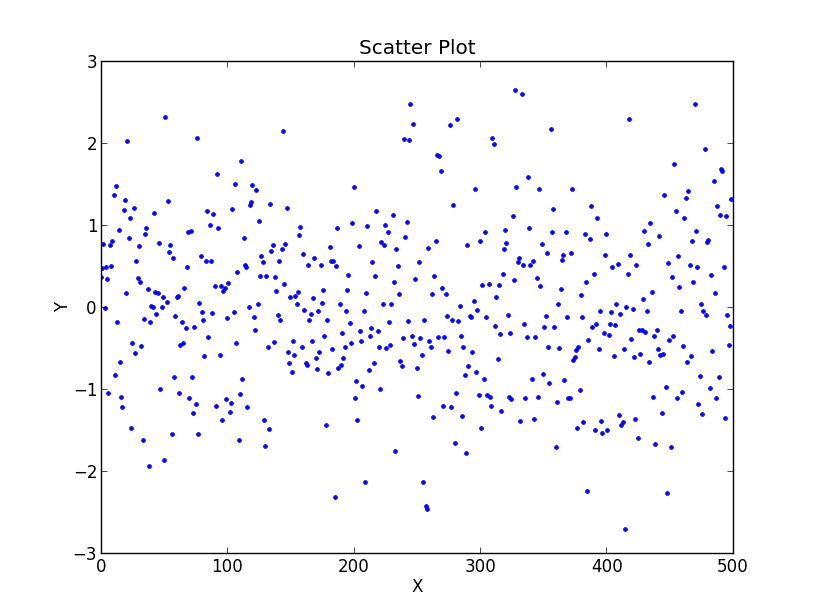
\includegraphics[width=0.5\textwidth]{../Images/scatterPlot.png}\\
  \caption{Scatter plot}
\end{figure}

\subsection{Histograms}\index{general}{plots!histogram}


\emph{Histograms} provide a first good overview of the distribution of your data.
If you divide by the overall number of data points, you get a \emph{relative frequency
histogram}; and if you just connect the top center points of each bin, you obtain a
\emph{relative frequency polygon}.

You can also smooth histograms with \emph{kernel-density-estimations (kde-plots)}. Those are nicely implemented and described in \emph{seaborn}.

\begin{figure}[ht]
  \centering
  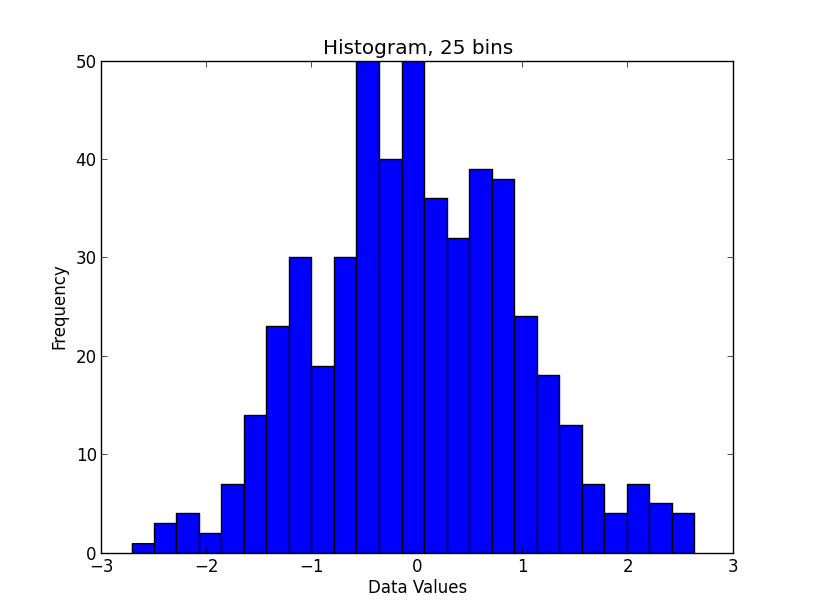
\includegraphics[width=0.5\textwidth]{../Images/Histogram.png}\\
  \caption{Histogram}
\end{figure}

\subsection{KDE-plots}\index{general}{plots!kde}

\footnote{This paragraph is taken from Wikipedia, "Kernel density estimation".} Kernel density estimates are closely related to histograms, but can be endowed with properties such as smoothness or continuity by using a suitable kernel. To see this, we compare the construction of histogram and kernel density estimators, using these 6 data points: x1 = −2.1, x2 = −1.3, x3 = −0.4, x4 = 1.9, x5 = 5.1, x6 = 6.2. For the histogram, first the horizontal axis is divided into sub-intervals or bins which cover the range of the data. In this case, we have 6 bins each of width 2. Whenever a data point falls inside this interval, we place a box of height 1/12. If more than one data point falls inside the same bin, we stack the boxes on top of each other.

For the kernel density estimate, we place a normal kernel with variance 2.25 (indicated by the red dashed lines) on each of the data points xi. The kernels are summed to make the kernel density estimate (solid blue curve). The smoothness of the kernel density estimate is evident compared to the discreteness of the histogram, as kernel density estimates converge faster to the true underlying density for continuous random variables.

\begin{figure}[ht]
  \centering
  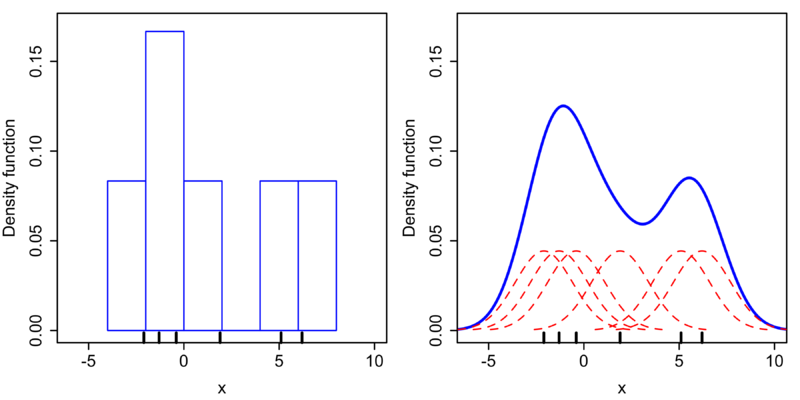
\includegraphics[width=0.75\textwidth]{../Images/Comparison_of_1D_histogram_and_KDE.png}\\
  \caption{Comparison of the histogram (left) and kernel density estimate (right) constructed using the same data. The 6 individual kernels are the red dashed curves, the kernel density estimate the blue curves. The data points are the rug plot on the horizontal axis. (from Wikipedia)}
\end{figure}

The bandwidth of the kernel is a free parameter which exhibits a strong influence on the resulting estimate. To illustrate its effect, we take a simulated random sample from the standard normal distribution (plotted at the blue spikes in the rug plot on the horizontal axis). The grey curve is the true density (a normal density with mean 0 and variance 1). In comparison, the red curve is undersmoothed since it contains too many spurious data artifacts arising from using a bandwidth h = 0.05 which is too small. The green curve is oversmoothed since using the bandwidth h = 2 obscures much of the underlying structure. The black curve with a bandwidth of h = 0.337 is considered to be optimally smoothed since its density estimate is close to the true density.

\begin{figure}[ht]
  \centering
  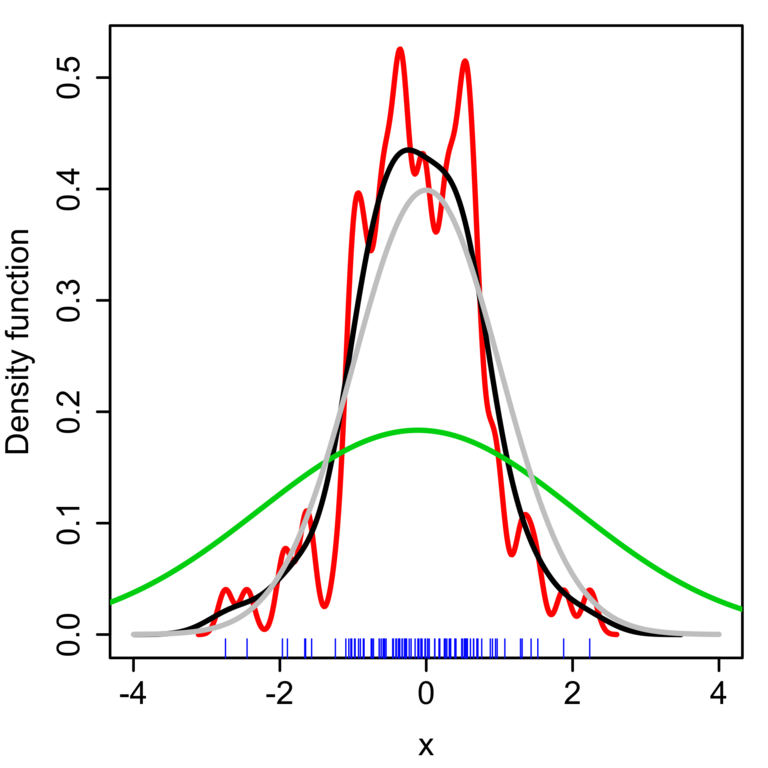
\includegraphics[width=0.5\textwidth]{../Images/Comparison_of_1D_bandwidth_selectors.png}\\
  \caption{Kernel density estimate (KDE) with different bandwidths of a random sample of 100 points from a standard normal distribution. Grey: true density (standard normal). Red: KDE with h=0.05. Green: KDE with h=2. Black: KDE with h=0.337. (from Wikipedia)}
\end{figure}

It can be shown that under certain conditions the optimal choice for h is
\begin{equation}
  h = \left(\frac{4\hat{\sigma}^5}{3n}\right)^{\frac{1}{5}} \approx 1.06 \hat{\sigma} n^{-1/5},
\end{equation}


where $\hat{\sigma}$ is the standard deviation of the samples.


\subsection{Cumulative Frequencies}\index{general}{cumulative frequency}

\emph{Cumulative frequency} curves indicate the number (or percent) of data with less than a given value. This is important for the statistical analysis (e.g. when we want to know the data range containing 95\% of all the values). Cumulative frequencies
are also useful for comparing the distribution of values in two or more different groups of individuals.

When you use percentage points, the cumulative frequency presentation has the additional advantage that it is bounded:

\begin{equation*}
  0 \leq x \leq 1
\end{equation*}

\begin{figure}[ht]
  \centering
  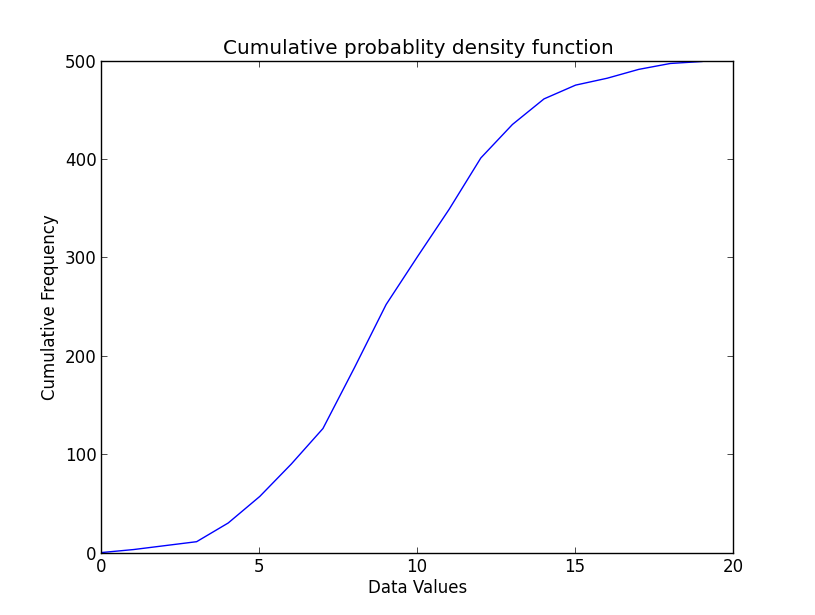
\includegraphics[width=0.5\textwidth]{../Images/CumulativeFrequencyFunction.png}\\
  \caption{Cumulative frequency function}
\end{figure}

\subsection{Box Plots}\index{general}{plots!boxplot}

\emph{Box plots} are frequently used in scientific publications to indicate values in two or more groups. The error bars typically indicate the \emph{range}. However, outliers are often excluded, and plotted separately. There are a number of tests to check for outliers. One of them is to check for data which lie more than 1.5 * \emph{inter-quartile-range} (IQR) above or below the first/third quartile (see Section \ref{sec:centiles}).

\begin{figure}[!ht]
  \centering
  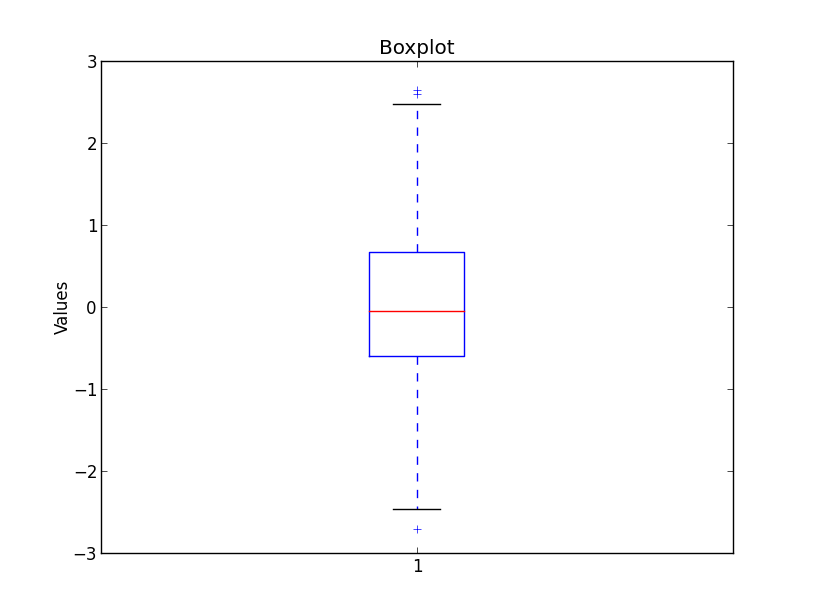
\includegraphics[width=0.5\textwidth]{../Images/boxplot.png}\\
  \caption{Box plot}\label{fig:Boxplot}
\end{figure}

Boxplots are often combined with KDE-plots to produce so-called \emph{violin-plots} \index{general}{plots!violinplot}, as shown in Figure \ref{fig:violin}.

\begin{figure}
  \centering
  % Requires \usepackage{graphicx}
  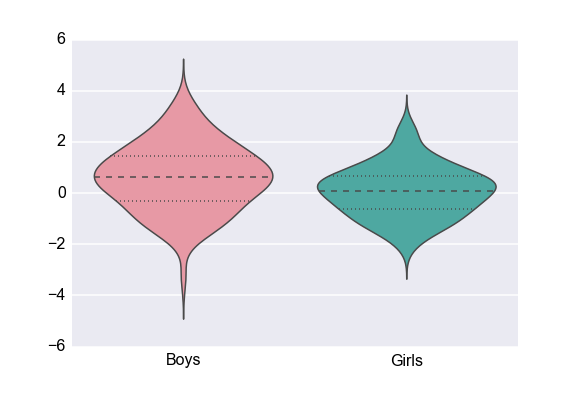
\includegraphics[width=0.75\textwidth]{../Images/violinplot.png}\\
  \caption{Violinplot, produced with \emph{seaborn}.}\label{fig:violin}
\end{figure}

\subsection{Programs: Data Display}
\PyImg "figsBasicPrinciples.py" (p \pageref{py:BasicPrinciples}) shows how the plots in this section have been generated.
\index{python}{figsBasicPrinciples}

\section{Study Design}


\subsection{Types of Studies}

\subsubsection{Observational or experimental}
With \emph{observational} studies the researcher only collects information, but does not interact with the study population. In contrast, in \emph{experimental} studies the researcher deliberately influences events (e.g. treats the patient with a new type of treatment) and investigates the effects of these interventions.

\subsubsection{Prospective or retrospective}
In \emph{prospective} studies the data are collected, starting with the beginning of the study. In contrast, a \emph{retrospective} study takes data acquired from previous events, e.g. routine tests taken at a hospital.

\subsubsection{Longitudinal or cross-sectional}
In \emph{longitudinal} investigations, the researcher collects information over a period of time, maybe multiple times from each patient. In contrast, in \emph{cross-sectional} studies individuals are observed only once. For example, most surveys are cross-sectional, but experiments are usually longitudinal.

\subsubsection{Case control and Cohort studies}
In \emph{case control} studies, first the patients are treated, and then they are selected for inclusion in the study, based on some characteristic (e.g. if they responded to a certain medication). In contrast, in \emph{cohort studies}, first subjects of interest are selected, and then these subjects are studied over time, e.g. for their response to a treatment.

\subsection{Design of Experiments}

\subsubsection{Bias} \index{general}{bias}
In general, when selecting our subject you try to make them representative of the population that you want to study; and you try to conduct your experiments in a way representative of investigations by other researchers. However, it is \emph{very} easy to get a \emph{bias} into your data. Bias can arise from a number of sources:
\begin{itemize}
  \item The selection of subjects.
  \item The structure of the experiment.
  \item The measurement device.
  \item The analysis of the data.
\end{itemize}
Care should be taken to avoid bias as much as possible.

\subsubsection{Randomized controlled trial} \index{general}{randomized controlled trial}
The gold standard for experimental scientific clinical trials is the \emph{randomized controlled trial}. Thereby bias is avoided by splitting the subjects to be tested into an \emph{intervention group} and a \emph{control group}\index{general}{control group}. The group allocation is made \emph{random}. By having the groups differ in only one aspect, i.e. is the factor \emph{treatment}, we should be able to detect the effect of the treatment on the patients.
Factors that can affect the outcome of the experiment are called \emph{covariates} or \emph{confoundings}. Through \emph{randomization}, covariates should be balanced across the groups.

\subsubsection{Randomization} \index{general}{randomization}
This may be one of the most important aspects of experimental planning. Randomization is used to avoid bias as much as possible, and there are different ways to randomize an experiment. For the randomization, \emph{random number generators}, which are available with most computer languages, can be used. To minimize the chance of bias, the randomly allocated numbers should be presented to the experimenter as late as possible.

Depending on the experiment, there are different ways to randomize the group assignment.

\paragraph{Simple randomization}
This procedure is robust against selection and accidental bias. The disadvantage is that the resulting groupsize can differ significantly.

For many types of data analysis it is important to have the same sample number in each group. To achieve this, other options are possible:

\paragraph{Block randomization}
This is used to keep the number of subjects in the different groups closely balanced at all times. For example, if you have two types of treatment, A and B, you can allocate them to two subjects in the following blocks:

\begin{enumerate}
  \item AABB
  \item ABAB
  \item ABBA
  \item BBAA
  \item BABA
  \item BAAB
\end{enumerate}

Based on this, you can use a random number generator to generate random integers between 1 and 6, and use the corresponding blocks to allocate the respective treatments. This will keep the number of subjects in each group always almost equal.

\paragraph{Minimization}
A closely related, but not completely random way to allocate a treatment is \emph{minimization}. Thereby you take whichever treatment has the smallest number of subjects, and allocate this treatment with a probability greater than 0.5 to the next patient.

\paragraph{Stratified randomization}
Sometimes you may want to include a wider variety of subjects, with different characteristics. For example, you may choose to have younger as well as older subjects. In that case you should try to keep the number of subjects within each \emph{stratum} balanced. For this you will have to keep different lists of random numbers for each group of subjects.

\subsubsection{Crossover studies} \index{general}{crossover studies}
An alternative to randomization is the \emph{crossover} design of studies. A crossover study is a longitudinal study in which subjects receive a sequence of different treatments. Every subject receives every treatment. To avoid causal effects, the sequence of the treatment allocation should be randomized.

\subsubsection{Blinding} \index{general}{blinding}
Consciously or not, the experimenter can significantly influence the outcome of an experiment. For example, a young researcher with a new "brilliant" idea for a new treatment will be bias in the execution of the experiment, as well in the analysis of the data, to see his hypothesis confirmed. To avoid such a subjective influence, ideally the experimenter as well as the subject should be blinded to the therapy. This is referred to as \emph{double blinding}. If also the person who does the analysis does not know which group the subject has been allocated to, we speak about \emph{triple blinding}.

\subsubsection{Replication} \index{general}{replication}
For variable measurements it is helpful to have a number of independent repetitions of each measurement.

\subsubsection{Sample selection} \index{general}{sample selection}
When selecting your subjects, you should take care of two points:

\begin{enumerate}
  \item Make sure that the samples are representative of the population.
  \item In comparative studies, care is needed in making groups similar with respect to known sources of variation.
\end{enumerate}

For example, if you select your subjects randomly from patients at a hospital, you automatically bias your sample towards subjects with health problems.

\subsubsection{Sample size}
Many studies fail, because the sample size is too small to observed an effect of the desired magnitude. To plan your sample size, you have to know
\begin{itemize}
  \item What is the variance of the parameter in the population you are investigating.
  \item What is the magnitude of the effect you are interested in, relative to the standard deviation of the parameter.
\end{itemize}

\subsection{Structure of Experiments}


In a designed experiment, there may be several conditions, called \emph{factors}\index{general}{factor}, that are controlled by the experimenter. If each combination of factors is tested, we talk about a \emph{factorial design} of the experiment.

In planning the analysis, you have to keep the important distinction between \emph{within subject} comparisons, and \emph{between subjects} comparisons.

%(Lecture 3)

\subsection{Data Management}

\subsubsection{Documentation} \index{general}{documentation}
Make sure that you document all the factors that may influence your results:

\begin{itemize}
  \item The date and time of the experiment.
  \item Information about the experimenters and the subjects.
  \item The exact paradigm that you have decided on.
  \item Anything noteworthy that happens during the experiment.
\end{itemize}

\subsubsection{Data Handling}
You can already significantly facilitate the data handling by storing your data with telltale names. For example, if you execute your experiments in Vienna and in Linz, you can store your rawdata with the format "[town][year][month][day].dat". For example, an experiment in Vienna on April 1, 2013 would be stored as "vi20130401.dat".

When you have finished recording the data, back up your data right away. Best do that into a directory that is separate from the one where you do your data analysis afterwards.

\subsection{Clinical Investigation Plan}

To design a medical study properly is not only advisable - it is even required by ISO 14155-1:2003, for \emph{Clinical investigations of medical devices for human subjects}. This norm specifies many aspects of your clinical study. It enforces the preparation of a \emph{Clinical Investigation Plan (CIP)}, specifying

\begin{enumerate}
  \item Type of study (e.g. double-blind, with or without control group etc.).
  \item Discussion of the control group and the allocation procedure.
  \item Description of the paradigm.
  \item Description and justification of primary endpoint of study.
  \item Description and justification of chosen measurement variable.
  \item Measurement devices and their calibration.
  \item Inclusion criteria for subjects.
  \item Exclusion criteria for subjects.
  \item Point of inclusion ("When is a subject part of the study?")
  \item Description of the measurement procedure.
  \item Criteria and procedures for the dropout of a subject.
  \item Chosen sample number and level of significance, and their justification.
  \item Procedure for documentation of negative effects or side-effects.
  \item List of factors that can influence the measurement results or their interpretation.
  \item Procedure for documentation, also for missing data.
  \item Statistical analysis procedure.
  \item The designation of a \emph{monitor} for the investigation.
  \item The designation of a \emph{clinical investigator}.
  \item Specification the data handling.
\end{enumerate}

\section{Exercises}

\begin{enumerate}
  \item
  \begin{enumerate}
    \item Read in the data from 'Data\textbackslash amst\textbackslash babyboom.dat.txt'.
    \item Inspect them visually, and give a numerical description of the data.
    \item Are the data normally distributed?
    \item How would you design the corresponding study?
  \end{enumerate}

\end{enumerate}


